\begin{Exercise}[title=Téleobjectif à deux miroirs]
Un téléobjectifs est constitué de deux miroirs un miroir concave $\mathcal{M}_1$ de focale 30cm percé d'un trou en son sommet $S_1$ et d'un miroir $\mathcal{M}_2$
\Question Quel est doit être le rayon de courbure de $\mathcal{M_2}$ pour que l'image d'un objet placé à l'infini sur l'axe se forme sur  le plan du film?
\Question Quel doit être le diamètre $d_2$ de $\mathcal{M}_2$ pour que tous les rayons réfléchis par $\mathcal{M}_1$ de diamètre $d_1$=10 cm soient collectés par $\mathcal{M}_1$
\Question Quelle doit être le diamètre $d_3$du trou pour que les rayons atteignent le film ? \\
\emph{Addenda} : Un miroir concave/convexe de rayon de courbure $R$ est équivalent à une lentille convergente/divergente de distance focale $f'= 2R$  accolé à un miroir en considérant un seul passage dans la lentille.
%\begin{figure}[h!]
\begin{center}
	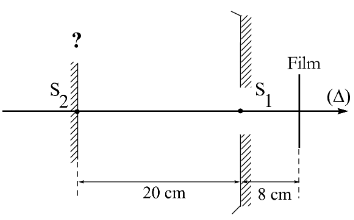
\includegraphics[scale=0.8]{./fig/teleob_vide.png}
\end{center}
%\end{figure}
\end{Exercise}
\begin{Answer}
\Question Le systeme optique considéré est : $A_\infty \xrightarrow[\mathcal{M}_1]{} F_1'=A' \xrightarrow[\mathcal{M}_2]{} A''_{\in \text{Film}}$
L’objet $A_\infty$ est à l’infini, son image intermédiaire est au foyer de $\mathcal{M}_1$,soit:
$\overline{S_1A'}=\overline{S_1F_1}=-30 cm$ d'où:
$\overline{S_2A'}=\overline{S_2S_1}+\overline{S_1A'}= -10cm$
De plus comme on veux $A''$ sur le film :
$\overline{S_2A''} = \overline{S_2S_1}+\overline{S_1A''}=28 cm $
Avec la relation de conjugaison pour $\mathcal{M}_2$
\[ \frac{1}{\overline{S_2A''}}+\frac{1}{S_2A'}=\frac{1}{f_2}=\frac{2}{\overline{S_2C_2}}\]
On obtient :
$S_2C_2=R_2= -31.1 cm$
\emph{Remarque} le miroir $\mathcal{M}_2$, pour la lumière incidente est un miroir concave (comme $M_1$), mais c’est en tant que miroir convexe qu’il est utilisé puisqu’il agit sur les rayons réfléchis par $M_1$
\Question Pour que tous les rayons réfléchis par $M_1$ soient collectés il faut qu'ils frappent tous $M_2$ pour ensuite revenir sur $M_1$ pour cela on doit avoir :
 $\tan \alpha =\frac{d_2}{2S_2A'}=\frac{d_1}{2S_1A'}$ \\
$d_2= d_1 \frac{S_2A'}{S_1A'}=3.33cm$

\Question Pour que tous les rayons atteignent le film il faut:
$\tan \alpha' = \frac{d_2}{2S_2A''}=\frac{d_3}{2S_1A''}$
\\
$d_3=d_2 \frac{S_1A''}{S_2A''}=0.95cm$
\begin{center}
	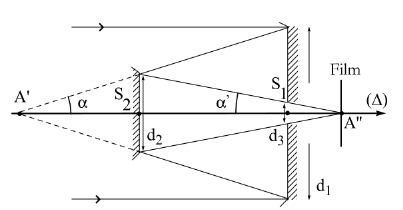
\includegraphics[scale=0.8]{./fig/teleob_plein.png}
\end{center}
\end{Answer}
